% ----------------------------------------------------------
% Histórico dos tipos de aplicações
% ----------------------------------------------------------
\chapter[Fundamentos]{Fundamentos}
%\addcontentsline{toc}{chapter}{Histórico}
% ----------------------------------------------------------

\section{IPC - Interprocess Communication}\label{sec:ipc}

Nem sempre um programa sequencial é a melhor solução para um determinado problema. Muitas vezes, as implementações são estruturadas na forma de várias tarefas inter-dependentes que cooperam 
entre si para atingir os objetivos da aplicação \cite{sistemas-op-mazierro}.

Diversos sistemas operacionais fornecem mecanismos para viabilizar a comunicação e o compartilhamento de dados entre aplicações. Coletivamente, as atividades habilitadas por estes mecanismos são chamadas de interprocess communications (IPC) \cite{microsoft-ipc}.

Os mecanismos que garantem a comunicação entre processos concorrentes e os acessos aos recursos compartilhados são chamados \textit{interprocess communication}. Algumas formas de IPC facilitam a divisão de trabalho entre diversos processos especialistas, enquanto outras facilitam esta divisão entre computadores dentro de uma rede.

Normalmente, os aplicativos que fazer parte de uma comunicação através de IPC são categorizados como clientes ou servidores. Um cliente é um aplicativo ou um processo que solicita um serviço de alguma outra aplicação ou processo. Por outro lado um servidor é um aplicativo ou um processo que responde a uma solicitação de cliente. Muitas aplicações agem como um cliente e servidor, dependendo da situação \cite{microsoft-ipc}.

A figura \ref{fig:how-communication-works} mostra como ocorre a comunicação entre processos (P1 e P2). Esta troca de informação pode acontecer de duas maneiras: em duas etapas, ou de forma direta. A comunicação em duas etapas envolve um processo coordenador, que pode ser um interpretador em Python utilizado para dar início ao \textit{workflow} por exemplo. A comunicação direta é ilustrada na figura ligada por linhas pontilhadas e não necessita de intermediação de nenhum processo. Esta maneira de comunicação pode ser executada através de diversas formas, entre elas: \textiit{Pipes}, \textiit{Shared Memory}, \textiit{Mapped Memory} e Arquivos compartilhados.

\begin{figure}[htbp]
    \centering
    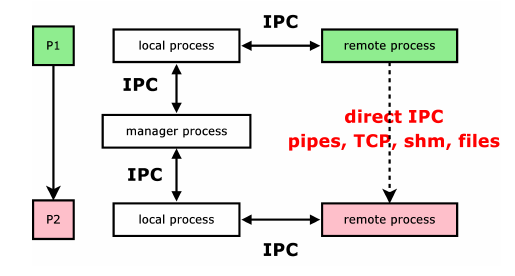
\includegraphics[width=1\textwidth]{figuras/ipc.png}
    \legend{Características dos mecanismos de comunicação \citeonline{sistemas-op-mazierro}}
    \label{fig:how-communication-works}
\end{figure}

\section{Cliente/Servidor}\label{sec:clientserver}

Também conhecido como arquitetura de duas camadas, o modelo cliente/servidor consiste em uma arquitetura em que a camada de apresentação se encontra no cliente e a camada de dados esta armazenada no servidor. Esta separação se opõe ao modelo centralizado amplamente utilizado até seu surgimento.

O processamento dos dados é dividido em duas partes distintas. Uma parte é a requerente de dados (cliente), e a outra parte é a provedora dos dados (servidor). O cliente envia durante sua execução uma ou mais solicitações ao servidor para realizar alguma tarefa específica. É dele a responsabilidade tanto de apresentar as informações para o usuário, quando executar as regras de negócio necessárias à aplicação. O servidor é responsável por armazenar os dados e prover um meio para que o cliente os consulte.

Desde a década de 1990, fornecedores de \textit{software} desenvolvem e trazem ao mercado muitas ferramentas para simplificar o desenvolvimento de aplicativos para a arquitetura cliente/servidor de 2 camadas. Algumas das mais conhecidas são: Microsoft Visual Basic, Delphi da Borland e PowerBuilder da Sybase. Estas ferramentas combinadas com milhões de desenvolvedores que sabem usá-las, significam que a abordagem de duas camadas cliente/servidor é uma solução econômica para certas classes de problemas.

Desde então, aplicações \textit{desktop} comunicando-se com o servidor de banco de dados se tornou um caso de uso normal. A maior parte da lógica de negócios foi incorporada dentro da aplicação \textit{desktop}. Portanto, esse estilo de clientes na aquitetura de duas camadas também foi chamado de \textit{fat clients}.

\begin{figure}[htbp]
    \centering
    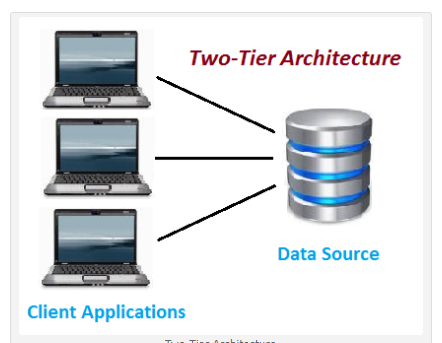
\includegraphics[width=0.5\textwidth]{figuras/two-tier.png}
    \caption{Comunicação em duas camadas}
    \label{fig:two-tier}
\end{figure}

A figura \ref{fig:two-tier} ilustra como a arquitetura em duas camadas funciona, mantendo uma comunicação direta entre cliente e servidor, sem intermediarios entre as duas pontas. Visto que neste modelo as regras de negócio estão presentes na camada de aplicação, ele é frequentemente aplicado em ambientes homogêneos. A camada de banco de dados e a camada de aplicação estão fisicamente próximos, o que oferece um bom desempenho para as aplicações.

Por outro lado, o modelo cliente servidor em duas cadamas possui grandes desafios de escalabilidade. Quando múltiplos usúarios executam requisições simultaneas, a aplicação perde muito desempenho, dado ao fato que cada cliente precisa de conecções separadas e memória de CPU para processar as requisições. Entretando, um dos maiores problemas na arquitetura em duas camadas ocorre quando há mudanças na estrutura do banco de dados. A maioria das aplicações cliente dependem da estrutura do banco de dados impedindo qualquer remodelagem, criando um problema de estruturas legadas, e muitas vezes subutilizadas.

Esta modelo foi substituido pelo modelo de três camadas, muito mais eficiente, e que fornece uma maneira de dividir as funcionalidades envolvidas na manutenção e apresentação de uma aplicação.

\section{Aplicações Monolíticas}\label{sec:monolitico}

Conforme \citeonline{monolithic-definition} explica, uma aplicação monolítica é construída como uma única unidade de \textit{software}. Estas aplicações são construídas em três partes: um banco de dados (que consiste em tabelas geralmente em um sistema de gerenciamento de banco de dados), uma interface de usuário do lado do cliente (consistindo de páginas executando em um navegador ou aplicativos móveis) e um lado do servidor de aplicação. Esta aplicação do lado do servidor tratará as requisições HTTP, executará a regra de negócio, recuperará e atualizará dados do banco de dados e construirá as respostas para serem enviadas às aplicações clientes. Estas camadas representam uma aplicação monolítica - um único executável lógico. Para fazer alterações no sistema, é necessário criar e implantar uma versão atualizada do aplicativo do lado do servidor.

Uma aplicação monolítica é autônoma e independente de outras aplicações. A filosofia do projeto consiste em um aplicativo que não é responsável apenas por uma determinada tarefa, mas que também pode executar todos os passos necessários para completar uma determinada função, como é mostrado na figura \ref{fig:three-tier}.

\begin{figure}[htbp]
    \centering
    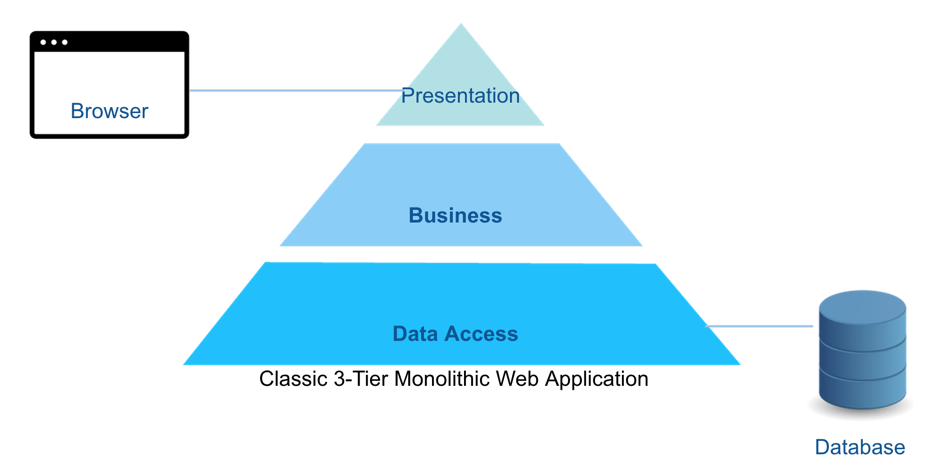
\includegraphics[width=0.5\textwidth]{figuras/three-tier.png}
    \caption{Aplicação monolítica clássica em 3 camadas}
    \label{fig:three-tier}
\end{figure}

\citeonline{monolithic-extinction} afirma que as aplicações monolíticas são uma maneira natural para a evolução de uma aplicação. A maioria das aplicações começam com um único objetivo, ou um pequeno número de objetivos relacionados. Ao longo do tempo, novas funcionalidades são adicionados ao aplicativo para suportar as necessidades do negócio. Entretando, as aplicaçõies monolíticas apresentam algumas desvantagens, sendo alguns deles: 

\begin{itemize}
    \item Um único ponto de falha pode comprometer o funcionamento correto de todos os módulos do sistema.
    \item Baixa estalabilidade dado a necessidade de copiar toda a \textit{stack} para escalar horizontalmente.
    \item Base de código \textbf{gigante}, uma vez que toda a regra de negócio se encontra em uma só base.
    \item É necessário muita comunicação para que várias equipes de desenvolvedores trabalhem em paralelo. Esta sobrecarga diminui o ritmo de desenvolvimento.
\end{itemize}

Contudo, com a popularização dos \textit{frameworks} Javascript como Angular e Backbone, houve um movimento de desacoplamento da camada de visualização nas aplicações monolíticas. Foram criadas então as chamadas aplicações \textit{frontend}, responsáveis pela camada de apresentação, e sendo executadas em dispositivos móveis como \textit{smartphones} e \textit{tables} ou nos \textit{browsers desktop}. 

Esse movimento criou um modelo monolítico de duas camadas, ilustrado na figura \ref{fig:two-tier-monolithic}. A remoção da interdependência entre as camadas de interface e servidor de aplicação facilitou o escalonamento e a escalabilidade de cada uma das partes. Esta separação de conceitos foi o primeiro passo em direção a uma arquitetura orientada a serviços.

\begin{figure}[htbp]
    \centering
    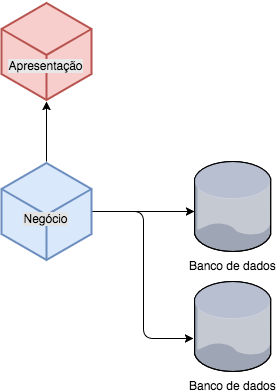
\includegraphics[width=0.5\textwidth]{figuras/two-tier-monolithic.png}
    \caption{Modelo monolítico de duas camadas}
    \label{fig:two-tier-monolithic}
\end{figure}

\section{SOA - Service Oriented Architecture}\label{sec:soa}

\citeonline{soa-cbdi} define SOA como políticas, práticas e frameworks que permitem que rotinas de aplicações sejam fornecidas e consumidas como conjuntos de serviços publicados em uma granularidade relevante para o consumidor do serviço. Os serviços podem ser invocados, publicados e descobertos e são abstraídos da implementação usando uma única forma de interface baseada em padrões.

Além de criar e expor serviços, \citeonline{soa-tech-target} assinala que o SOA tem a capacidade de aproveitar esses serviços de forma recursiva em aplicações (conhecidos como aplicativos compostos). O SOA vincula esses serviços à orquestração ou alavanca individualmente esses serviços. Desta forma, o SOA é visto como uma evolução das arquiteturas existentes, abordando a maioria dos principais sistemas como serviços e resgatando esses serviços em um único domínio onde eles formam soluções.

 O SOA permite a reutilização de ativos existentes, onde novos serviços podem ser criados a partir de uma infra-estrutura de sistemas de TI existente. Em outras palavras, ele permite que as empresas reutilizem aplicativos existentes e possibilita a interoperabilidade entre aplicações e tecnologias heterogêneas. Ele fornece um nível de flexibilidade que não era possível antes, no sentido de que:

\begin{itemize}
    \item Os serviços são componentes de software com interfaces bem definidas que são independentes da implementação. Um aspecto importante do SOA é a separação da interface de serviço (o que) da sua implementação (como). Esses serviços são consumidos por clientes que não estão preocupados com a forma como esses serviços irão executar suas solicitações;
    \item Os serviços são autônomos (executar tarefas predeterminadas) e vagamente acoplados (para independência);
    \item Serviços compostos podem ser construídos a partir de agregados de outros serviços;
\end{itemize}

Isso significa que o SOA é uma abordagem alinhada com o negócio, em que os aplicativos dependem dos serviços disponíveis para facilitar os processos de negócios. Um serviço é um componente de \textit{software} reutilizável e autônomo, fornecido por um provedor de serviços e consumido pelos solicitantes. O SOA cria uma visão de flexibilidade de TI que facilita a agilidade do negócio. Sua implementação envolve principalmente componentes de aplicativos corporativos e/ou em desenvolvimento que usam serviços, disponibilizando aplicativos como serviços para outras aplicações \cite{soa-book}.

\begin{figure}[htbp]
    \centering
    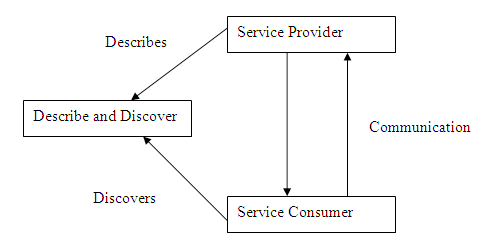
\includegraphics[width=0.5\textwidth]{figuras/soa.png}
    \caption{Service Oriented Architecture}
    \label{fig:soa}
\end{figure}

\citeonline{soa-intel} acrescenta que em um ambiente SOA típico, existe um provedor de serviços e um consumidor de serviços. Para que isso funcione, também é necessário um mecanismo para que eles possam se comunicar uns com os outros, como é ilustrado na figura \ref{fig:soa}. A W3C \footnote{World Wide Web Consortium} definiu um padrão aberto para que \textit{web services} possam implementar o SOA e habilitar a comunicação entre o provedor e o consumidor através de um protocolo baseado em XML: o \textit{Simple Object Access Protocol} (SOAP). Outros padrões também são usandos ou foram criados para realizar a comunicações entre os serviçoes SOA. Alguns basearam-se no \textit{design} do \textit{REpresentation State Transfer} (REST), utilizando tanto XML quando JSON para transportar os dados entre os serviços.

Em geral, há uma confusão entre o relacionamento entre SOA e \textit{web services}. \citeonline{soa-webservice} faz uma distinção entre o SOA e \textiit{web services} do seguinte modo: \"Web services tratam-se de especificações de tecnologias, enquanto o SOA é um princípio de \textit{design} de \textit{software}. Notavelmente, Web services são um padrão de definição de interface adequado ao SOA e é neste ponto onde eles se conectam ao SOA". Portanto, o SOA é um padrão de arquitetura, enquanto os \textit{Web services} são serviços implementados usando um conjunto de padrões. Os \textit{Web services} são uma das maneiras em que é possível implementar o SOA. cujo os benefícios são que é possível alcançar uma abordagem neutra em relação a plataformas para acessar serviços e uma melhor interoperabilidade à medida que mais fornecedores suportam cada vez mais especificações.
